\documentclass[fleqn]{VUMIFKompMagistrinis}
\usepackage{algorithmicx}
\usepackage{algorithm}
\usepackage{algpseudocode}
\usepackage{amsfonts}
\usepackage{amsmath}
\usepackage{bm}
\usepackage{caption}
\usepackage{color}
\usepackage{float}
\usepackage{graphicx}
\usepackage{listings}
\usepackage{subfig}
\usepackage{wrapfig}

% Titulinio aprašas (nereikalingus elementus užkomentuoti)
\university{Vilniaus universitetas}
\faculty{Matematikos ir informatikos fakultetas}
\institute{Informatikos institutas}  % Užkomentavus šią eilutę - institutas neįtraukiamas į titulinį
\department{Programų sistemų BAKALAURO STUDIJŲ PROGRAMA}
\papertype{Kursinis darbas}
\title{Ligų aptikimas naudojant plaučių echoskopiją}
\titleineng{Detecting diseases with lung ultrasound}
\author{Justas Baniulis}
\status{4 kurso, 1 grupės studentas}
% \secondauthor{Vardonis Pavardonis}   % Pridėti antrą autorių
% \thirdauthor{Vardonis Pavardonis}   % Pridėti antrą autorių
% \fourthauthor{Vardonis Pavardonis}   % Pridėti antrą autorių
\supervisor{asist. dr. Tomas Plankis}
% \reviewer{doc. dr. Vardauskas Pavardauskas}
\date{Vilnius \\ \the\year}

% Nustatymai
% \setmainfont{Palemonas}  % Pakeisti teksto šriftą į Palemonas (turi būti įdiegtas sistemoje)
\bibliography{bibliografija}  % Literatūros šaltinių aprašų failas bus bibliografija.bib

\begin{document}
\maketitle

\tableofcontents

% \santrauka{Santrauka}
% Glaustai aprašomas darbo turinys: pristatomi darbo tikslai, analizuotos ir
% tirtos problemos, atlikti eksperimentai bei padarytos išvados, gautos
% rekomentacijos. Santraukos apimtis ne didesnė nei 0,5 puslapio. Santraukų gale
% nurodomi darbo raktiniai žodžiai. 
% Nurodomi iki 5 svarbiausių temos raktinių žodžių (terminų).
% Vienas terminas gali susidėti iš kelių žodžių.
% \raktiniaizodziai{raktinis žodis 1, raktinis žodis 2, raktinis žodis 3, raktinis žodis 4, raktinis žodis 5}

\sectionnonum{Įvadas}
Plaučių echoskopija yra plaučių tyrimas, kuris vizualizuoja plaučių organo artefaktus naudodamas aukšto dažnio garso bangas. Sveikatos priežiūros specialistas ant paciento krūtinės naudoja echoskopijos įrenginį, kuris skleidžia garso bangas. Šios bangos atšoka ir tas pats įrenginys jas surenka. Bangos atšoka skirtingai nuo skirtingų medžiagų, kaip oras, skystis, audiniai ir galutiniame echoskopijos rezultate matomi skirtingai atšokusių garso bangų suformuoti artefaktai (žr. \ref{img:plauciai_art} paveikslėlį). Plaučių echoskopijos tyrime yra nagrinėjami artefaktai, kaip A linijos, B linijos, konsolidacijos ir pleuros ertmės (linijos). Naudojantis pastebimais artefaktais, gydytojas gali diagnozuoti ligas ar nusatyti sveikus plaučius (žr. \ref{tab:ligos} lentelę)
\begin{figure}[H]
    \centering
    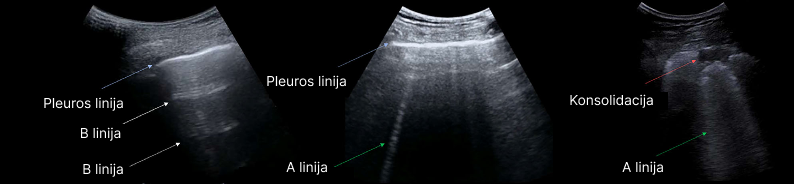
\includegraphics[scale=0.5]{img/plauciai_artefaktai.png}
    \caption{Plaučių artefaktų pavyzdžiai \cite{demi2023new}}
    \label{img:plauciai_art}
\end{figure}\begin{table}[H]\footnotesize
  \centering
  \caption{Echoskopijos artefaktų ir ligų sąryšis \cite{demi2023new, cammarota2023lung}}
  \begin{tabular}{|l|c|c|c|c|c|} \hline
     Artefaktas & Galimos diagnozės \\
    \hline
    A linija  & Sveiki plaučiai \\
    B linija & Širdies ydos, COVID-19, virusinis plaučių uždegimas, plaučių edema \\
    Konsolidacija & Bakterinis plaučių uždegimas, atelektazė, plaučių sumušimas \\
    Pleuros linija & Pneumotoraksas, pleuros efuzija, pleuros fibrozė \\
    \hline
  \end{tabular}
  \label{tab:ligos}
\end{table}
\par
Šis tyrimas paskutinį dešimtmetį tampa vis dažniau naudojamas sveikatos priežiūros specialistų \cite{demi2023new}. Plaučių echoskopija yra patrauklus naudoti tyrimas, nes jo kaina mažesnė už įprastai naudojamus rentgeno ar tamografijos tyrimus, paciento nereikia transportuoti į radiologinį skyrių, echoskopijos prietaisai neskleidžia žmogui pavojingos radiacijos, patyręs profesionalas gali interpretuoti echoskopiją efektyviau negu rentgeno nuotraukas ir greičiau, nes echoskopijos prietaisai veikia realiu laiku. Šio tyrimo trūkumas yra tai, kad išmokti interpretuoti echoskopijos rezultatus yra sunku, užtrunka laiko ir žmogiškųjų išteklių perduoti įgytai patirčiai \cite{cammarota2023lung}.

% Įvade aprašomi darbo tikslai, 
Specialistams ligos diagnozavimo darbą su plaučių echoskopija gali palengvinti dirbtinis intelektas \cite{demi2023new}. Šio darbo tikslas yra apžvelgti ir palyginti klasifikacinius giliojo mokymosi tinklus, kurie nustato ligos diagnozę naudojantis echoskopinėmis nuotraukomis. 
% nurodomas temos aktualumas, motyvacija,
% formuluojamas sprendžiamas uždavinys ir siekiami rezultatai.

% Aptariamos teorinės darbo prielaidos bei metodika, apibrėžiamas tiriamasis
% objektas, apibūdinami su tema susiję literatūros ar kitokie šaltiniai, temos
% analizės tvarka, darbo atlikimo aplinkybės


\section{Transformerių neuroninis tinklas}
2021 metų rugsėjį elektrotechnikos ir elektronikos inžinierių instituto (angl. IEEE) konferencijos „IEEE International Conference on Image Processing“ publikuotame straipsnyje „POCFormer: A Lightweight Transformer Architecture for Detection of COVID-19 Using Point of Care Ultrasound“ autoriai sukūrė neuroninio tinklo architektūrą, kuri geba klasifikuoti plaučių echoskopijos nuotraukas\cite{PAY21}. Pasak straipsnio autorių, COVID-19 diagnozė naudojantis patvirtintomis priemonėmis, kaip PGR tyrimai, nors ir yra labai tiksli, tačiau užtrunka labai daug laiko ir dėl to negali būti naudojamos dideliu mastu. Pagal straipsnio autorius, technologiškai patobulinti mobilūs echoskopijos įrenginiai leidžia greičiau ir patogiau išgauti echoskopinę nuotrauką ir jie yra vis dažniau naudojami tarp sveikatos priežiūros specialistų. Straipsnio autoriai teigia, kad šių mobilių echoskopijos įrenginių trūkumas yra tai, kad gautus echoskopijos rezultatus gali analizuoti ir ligą diagnozuoti tik labai patyręs specialistas, o įgauti patirtį užtrunka laiko ir yra sunku. Straipsnio autoriai, kad palengvintų sveikatos priežiūros specialistų darbą interpretuojant gautas nuotraukas, automatizavo COVID-19 ir bakterinio plaučių uždegimo nustatymą iš echoskopinės nuotraukos. Apžvelgsime straipsnio autorių sukūrtą klasifikacijos modelį „POCFormer“, paremtą transformerių neuroninio tinklo architektūra, ir klasifikuojantį nuotrauką į COVID-19, bakterinio plaučių uždegimo, sveikų plaučių klases. \cite{PAY21}

\subsection{Architektūra}

Autorių sukurtą modelį sudaro dvi pagrindinės dalys: 
\begin{enumerate}
    \item Regos tranformerių neuroninis tinklas (angl. „Vision transformer“, sutrumpinimas „ViT“), kuris išekstrahuoja požymius iš suskaidytos echoskopinės nuotraukos derinant tos nuotraukos dalis su pozicijos įterpiniais \cite{PAY21}. Ši dalis aprašoma plačiau \ref{sec:vit} skyriuje.
    \item Tiesinis tranformerių neuroninis tinklas (angl. „linear transformer“, sutrumpinimas „Linformer“), kuris atlieka požymių, gautų iš „Vision transformer“ enkodinimą \cite{PAY21}. Ši dalis aprašoma plačiau \ref{sec:linformer} skyriuje.
\end{enumerate}
\par
Modelis taip pat turi du mažesnius sluoksnius:
\begin{enumerate}
    \item Prieš paduodant tranformerių neuroniniui tinklui nuotrauką, pirmame sluoksnyje ji yra suskaidoma į atskiras dalis. Tuomet dalys ištiesinamos, sukuriama dalių linijinė projekcija ir gauti vektoriai perduodami transformerių blokams. \cite{PAY21}
    \item Architektūroje egzistuoja paskutinysis „tankusis“ (arba pilnai sujungtų sąryšių) sluoksnis, kuris priima „Vision transformer“ ir „Linformer“ transformerių tinklų požymius ir paverčia juos klasių (COVID-19, bakterinis plaučių uždegimo, sveikų plaučių) išeitimi. \cite{PAY21}
\end{enumerate}
Aukšto lygio „POCFormer" modelio architektūra iliustruota \ref{img:POCFormer} paveikslėlyje .
\begin{figure}[H]
    \centering
    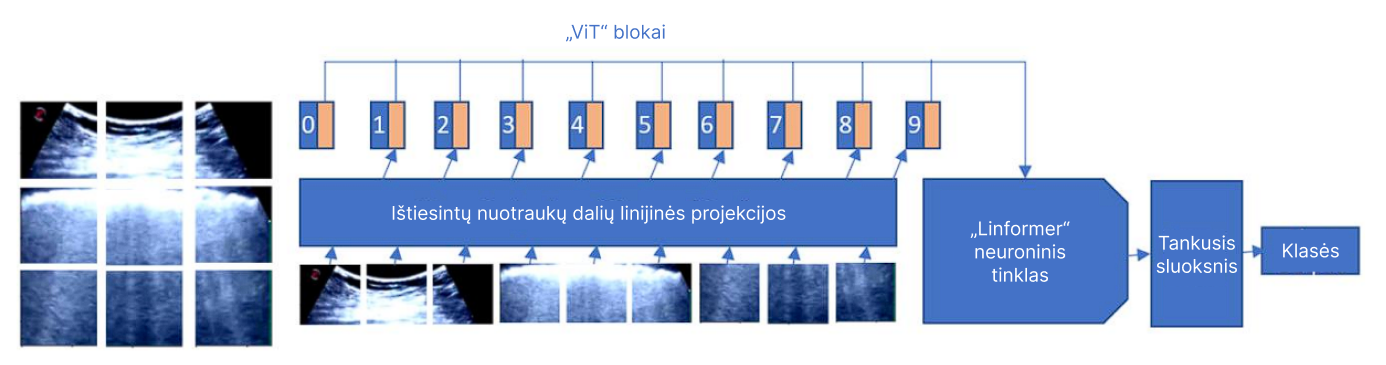
\includegraphics[scale=0.45]{img/transformerisMain.png}
    \caption{Aukšto lygio „POCFormer" modelio architektūra \cite{PAY21}}
    \label{img:POCFormer}
\end{figure}

\subsubsection{„ViT“ dalis}
\label{sec:vit}
\par
Pirmasis transformerių neuroninis tinklas buvo pristatytas 2017 metais „Attention is All You Need“ straipsnyje. Šio straipsnio autorių sukurta neuroninio tinklo architektūra skirta skaitmeniniam natūraliosios kalbos apdorojimui - dėmesio sutelkimo mechanizmas leidžia modeliui suprasti sąryšius tarp skirtingų tekstinių duomenų dalių ir suprasti kontekstą bei sąryšius jose. \cite{tranformeris}
\par
„Vision transformer“ modelis buvo pristatyas 2021 metų straipsnyje „An Image is Worth 16x16 Words: Transformers for Image Recognition at Scale“. Pasak šio straipsnio autorių, transformerių neuroninis tinklas gali būti naudojamas ne tik skaitmeniniam natūraliosios kalbos apdorojimui, bet ir nuotraukų klasifikacijos uždaviniams \cite{dosovitskiy2021image}. „Vision transformer“ modelis nuotrauką suskaido į atskiras dalis ir jos linijine projekcija sudedamos į vektorių kartu su pozicijos įterpiniu, kad modelis žinotų dalių originalią poziciją. Modelio pagrindinė dalis yra enkodinimo blokas, kurį sudaro keli dėmesio sutelkimo sluoksniai ir daugiasluoksnio perceptrono blokai. Dėmesio sutelkimo mechanizmas, kaip ir skaitmeniniame natūraliosios kalbos modelyje, leidžia modeliui įvertinti atskirų nuotraukų dalių globalius kontekstinius ryšius bei lokalųjį kontekstą. Taip pat prieš daugiasluoksnio perceptrono blokus yra du sluoksniai su gausinio tiesinio vieneto (angl. sutrumpinimas „GELU“) aktyvacijos funkcija, kuri leidžia tinklui mokintis sudėtingus šablonus (žr. formulę \ref{eq:gelu}) ir sluoksnio normalizacija (angl. sutrumpinimas „LayerNorm“) (žr. formulę \ref{eq:layernorm}), kuri stabilizuoja neuroninį tinklą normalizuojant kiekvieno sluoksnio požymių įvestis. Blokus seka praleidimo jungtys, kurios padeda išspręsti nykstančio gradiento problemą. \cite{dosovitskiy2021image}
\begin{equation}
    \centering\label{eq:gelu}
    \text{GELU}(x) = x \Phi(x)
\end{equation}
\par
\(\Phi(x)\) - normalaus atsitiktinio dydžio pasiskirstymo funkcija. 
\begin{equation}\label{eq:layernorm}
    \centering
    \text{LayerNorm}(x) = \gamma \odot \frac{x - \mu}{\sqrt{\sigma^2 + \epsilon}} + \beta
\end{equation}
\par
\( x \) - įvesties vektorius, t.y sluoksnio išvestis prieš normalizaciją.
\( \mu \) ir \( \sigma^2 \) - vidurkis ir variacija, apskaičiuojami kiekvieno duomenų taško požymių ašyse.
\( \epsilon \) - maža konstanta skaitmeniniam stabilumui užtikrinti, užkerta kelią dalybai iš nulio, kai variacija yra labai maža.
 \( \gamma \) ir \( \beta \) - mokomi „LayerNorm“ parametrai mastelio ir poslinkio keitimui. Rreguliuojami mokymo proceso metu.
\( \odot \) - elementų pagal elementus dauginimas.

\par
Transformerių neuroninių tinklų architektūra geba, pagal kūrėjus, per mažesnį epochų skaičių ir su mažiau duomenų gali pasiekti ir kai kuriuose uždaviniuose pralenkti konvoliucinių neuroninų tinklų (angl. CNN) architektūrų, kurios dažniausiai naudojamos nuotraukų klasifikacijai, metrikas \cite{dosovitskiy2021image}. Kadangi plaučių echoskopinių nuotraukų straipsnio rašymu metu buvo trūkumas, ši architektūra padėjo išspręsti mažo duomenų kiekio problemą. \cite{PAY21}   
\subsubsection{„Linformer“ dalis}
\label{sec:linformer}
Nors transformerių neuroninių tinklai prilygsta ar yra geresni CNN metrikų atžvilgiu, šių tinklų treniravimas ir naudojimas užima daug resursų dėl „Vision transformer“ dėmesio sutelkimo enkoderio sudėtingumo. Didelis parametrų skaičius apsunkina mobilių echoskopijos prietaisų darbą, nes jų atmintis ir skaičiavimo pajėgumai yra stipriai apriboti \cite{PAY21}. Dėl šios priežasties kūrėjai pasinaudojo „Linformer“ enkoderiu, 2020 metais pristatytu „Linformer: Self-Attention with Linear Complexity“ straipsnyje, kuris optimizavo tranformerių dėmesio sutelkimo mechanizmą. \cite{PAY21, wang2020linformer}.
\par
Pasak „Linformer“ enkoderio autorių, jų dėmesį sutelkančio mechanizmo sudėtingumas yra \( O(n) \), o originalaus „Vision transformer“ sudėtingumas yra \( O(n^2) \) laiko ir atminties atžvilgiu \cite{wang2020linformer}. Straipsnio autoriai sugebėjo optimizuoti enkodinimą aproksimuojant dėmesio sutelkimo mechanizmą su žemo rango matricos faktorizacija, parametrų dalinimusi tarp komponentų ir pridedant dvi linijines projekcijas apskaičiuojant reikšmes \cite{wang2020linformer}. Vieno komponento architektūra iliustruota paveiklėlyje \ref{img:linformer}.

\begin{figure}[H]
    \centering
    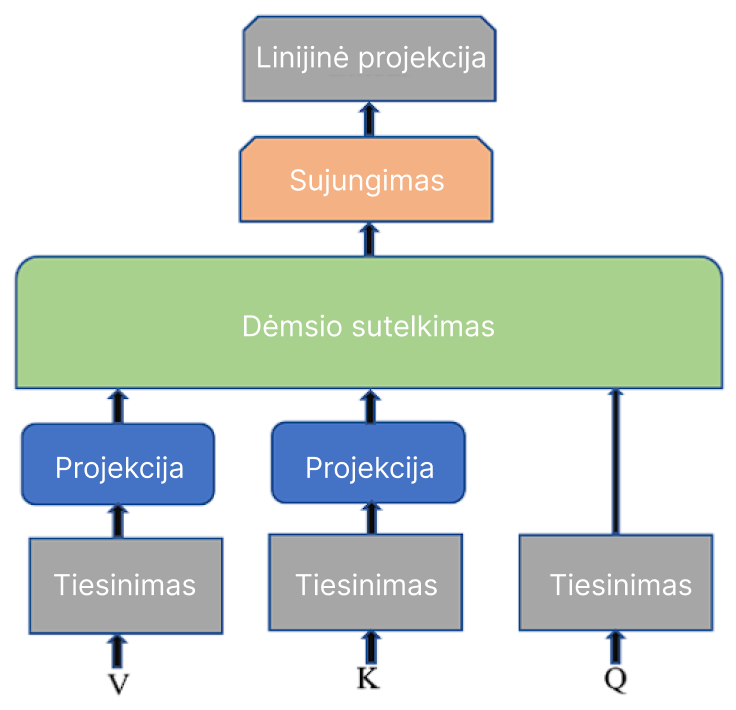
\includegraphics[scale=0.40]{img/linformer.PNG}
    \caption{Vieno „Linformer" komponento architektūra \cite{PAY21}}
    \label{img:linformer}
\end{figure}

\par
Pagal „POCFormer" modelio autorius, jų modelis, naudojantis „Linformer“ metodą, turi ženkliai mažesnį parametrų kiekį palyginus su kitais nuotraukų klasifikacijos ir skaitmeninio kalbos apdorojimo modeliais, paremtais transformerių neuroniniais tinklais (žr. lentelę \ref{tab:parametrai1}), o tai labai svarbu mobiliems echoskopijos prietaisams su ribotais resursais ir siekiant sveikatos priežiūros specialistams greitai nustatyti ligą. Be to, šis sprendimas, pasak autorių, leidžia naudotis tranformerių neuroninių tinklų mokymosi su lokaliais ir globaliais kontekstiniais ryšiais savybe, kuri svarbi išlaikant aukštas metrikas nuotraukų klasifikacijoje ir nustatant ligą. \cite{PAY21}

\begin{table}[H]\footnotesize
  \centering
  \caption{Transformerių neuroninių tinklų palyginimas \cite{PAY21, dosovitskiy2021image}}
  \begin{tabular}{|l|c|c|} \hline
    Modelis    & Parametrų kiekis \\
    \hline
    „BERT“ & \( 345 \cdot 10^6 \) \\
    „Vision transformer“ & \( \approx61 \cdot 10^6 \) \\
    \textbf{„POCFormer" daugelio klasių}  & \( \textbf{6.9} \cdot \textbf{10} ^ \textbf{6} \) \\
    \hline
  \end{tabular}
  \label{tab:parametrai1}
\end{table}

\subsection{Duomenys}
Autoriai teigia, jog modelio treniravimui naudojo atviros prieigos duomenų rinkinį, kuriame saugomi medicinos ekspertų sužymėti plaučių echoskopijos vaizdo įrašai ir nuotraukos iš pacientų\cite{PAY21}. Pasak autorių, treniravimo ir testavimo duomenų rinkiniai buvo sukurti naudojantis plaučių echoskopijos vaizdo įrašų kadrais ir nuotraukomis, kurie suskirstyti į tris kategorijas - COVID-19, bakterinio plaučių uždegimo ir sveikų plaučių. Pagal autorius, kad treniravimo, validacijos ir testavimo duomenų rinkinių klasės būtų subalansuotos, modelio nuostolių funkcijoje buvo panaudotas parametrų balansavimo mechanizmas (žr. formulę \ref{eq:weight_vector}), kuris parametrų vektoriuose klasėms, kurios turi mažiau duomenų, suteikia aukštesnę parametro reikšmę.\cite{PAY21}
\begin{equation}\label{eq:weight_vector}
    \text{weight\_vector} = \frac{1}{X/\min(X)}
\end{equation}
\( X \) - kiekvienos klasės nuotraukų kiekis
\par
Pagal autorius, dažniausiai pasitaikantys echoskopinių vaizdo įrašų kadrų ir nuotraukų požymiai yra A ir B linijos. Išgautiems kadrams, prieš pradedant treniravimą, autoriai pritaikė šias transformacijas, kad nuotraukos gautos iš skirtingų šaltinių būtų standartizuotos \cite{PAY21}:
\begin{enumerate}
    \item konvertuojamos nuotraukos į 224 \(\cdot\) 224 dimensiją.
    \item 8 bitų nuotraukoms atliekama normalizacija tarp reikšmių \([0,1]\) 
    \item nuotraukų vidurkis ir standartinis nuokrypis perskaičiuojami (žr. formules \ref{eq:transformerio}) 
\end{enumerate}
\begin{equation}\label{eq:transformerio}
\mu = \left( \frac{1}{n} \sum_{i=1}^{n} x_i \right), \quad
\sigma = \sqrt{\frac{1}{N} \sum_{i=1}^{N} (x_i - \mu)^2}
\end{equation}
\( x_i = [R_i, G_i, B_i]^T \) - raudonos, geltonos, mėlynos spalvos kanalai, \(\mu\) - nuotraukos vidurkis, \(\sigma\) - nuotraukos standartinis nuokrypis. 
\par
Straipsnio autoriai iš duomenų rinkinio priskyrė \(\approx400\) nuotraukų kiekvienai klasei. Toks, pagal autorių nuomone, mažas kiekis buvo pasirinktas norint pademonstruoti architektūros gebėjimą pasiekti aukštas metrikas naudojantis mažesniu duomenų rinkiniu, kadangi surinkti didelius duomenų kiekius medicinos srityje yra sunku, nes rinkimas reikalauja daug pastangų.\cite{PAY21}
\subsection{Apmokymas}
Straipsnio autoriai treniravo keturis klasifikacijos modelius - tris dviejų klasių klasifikavimo ir vieną daugelio klasių klasifikavimo \cite{PAY21}. Straipsnio autorių dvejų klasių modeliai susidaro iš:
\begin{enumerate}
    \item COVID-19 ir sveikų plaučių klasifikacija,
    \item COVID-19 ir bakterinio plaučių uždegimo klasifikacija,
    \item Bakterinio plaučių uždegimo ir COVID-19 klasifikacija
\end{enumerate}
\par 
Autoriai teigia jog, vykstant treniravimo procesui jie ieškojo geriausių hiperparametrų, kadangi „Vision transformer“ tinklas ir „Linformer“ modelis turi efektyviai veikti kartu \cite{PAY21}. Taip pat autoriai teigia, jog dviejų klasių modelių kūrimas ir sėkmingas treniravimas jiems padėjo parinkti hiperparametrų reikšmes ir daugelio klasių modeliui. Autorių pateikti naudojami hiperparametrai modeliuose pateikti \ref{tab:parametrai1} lentelėje. Mokymo epochų kiekio autoriai nepateikia. 
\begin{table}[H]\footnotesize
  \centering
  \caption{„POCFormer“ hiperparametrai \cite{PAY21}}
  \begin{tabular}{|l|c|c|} \hline
     & Daugelio klasių & Dvejų klasių \\
    \hline
    Sluoksnių kiekis &  32&  12 \\
    Paslėptų sluoksnių dydis &  64&  32 \\
    Daugiasluoksnio perceptrono dydis &  128&  128 \\
    Nuotraukos dalies dydis &  32&  32 \\
    Dėmesio sutelkimo „galvutės“ &  8&  8 \\
    Parametrų kiekis &  6,9 mln.&  2,8 mln. \\
    \hline
  \end{tabular}
  \label{tab:parametrai1}
\end{table}
\par
Autoriai treniravimui, validacijai ir testavimui naudojo PyTorch karkasą ir nuosavus kompiuterinius resursus, kuriuos sudarė Intel Core i7-9700K 4.7GHz procesorius ir RTX 2080 vaizdo plokštė su 8GB RAM. „POCFormer“ modelio kaštų funkcija yra kryžminės entropijos funkcija (žr. formulę \ref{eq:cross}) \cite{PAY21}.\begin{equation}\label{eq:cross}
\text{Cross Entropy Loss} = - \sum_{c=1}^{M} y_{o,c} \log(p_{o,c})
\end{equation}
\( p \) - prognozuojama tikimybė, jog stebimasis \(o\) priklauso \(c\)  klasei, o \(y\) yra dvejetainis rodiklis (0 arba 1), nusakantis ar klasė \(c\) yra teisingai klasifikuojama stebimam \(o\) \cite{PAY21}.
\subsection{Rezultatai}
Straipsnio autoriai ištreniruotų dvejų klasių modelių efektyvumui vertinti naudojo preciziškumo, tikslumo, F1, jautrumo ir specifiškumo  metrikas (žr. \ref{tab:statistikos1} lentelę) ir daugelio klasių modelio efektyvumui vertinti naudojo atkūrimo, preciziškumo, F1, specifiškumo ir jautrumo metrikas (žr. \ref{tab:statistikos2} lentelę ). 
\par
Straipsnio autorių modeliai efektyviai klasifikuoja COVID-19, bakterinio uždegimo ir sveikų plaučių klases - visų metrikų reikšmės yra aukštos. Aukštos preciziškumo ir tikslumo reikšmės rodo, jog modelis pateikia mažai klaidingai teigiamų ir klaidingai neigiamų spėjimų. Visuose modeliuose aukštas F1 rodo, jog architektūra yra gerai subalansuota.
\begin{table}[H]\footnotesize
  \centering
  \caption{„POCFormer“ dvejų klasių modelių metrikos \cite{PAY21}}
  \begin{tabular}{|l|c|c|c|c|c|} \hline
    Modelis & Preciziškumas & Tikslumas & F1 & Jautrumas & Specifiškumas \\
    \hline
    COVID-19 ir sveiki plaučiai & 0.87 & 0.91 & 0.92 & 0.83 & 0.97 \\
    COVID-19 ir bakterinis uždegimas & 0.93 & 0.95 & 0.93 & 1.00 & 0.88 \\
    Bakterinis uždegimas ir sveiki plaučiai & 0.95 & 0.95 & 0.93 & 1.00 & 0.80 \\
    \hline
  \end{tabular}
  \label{tab:statistikos1}
\end{table}\begin{table}[H]\footnotesize
  \centering
  \caption{„POCFormer“ daugelių klasių modelio metrikos \cite{PAY21}}
  \begin{tabular}{|l|c|c|c|c|c|} \hline
     Klasė & Atkūrimas & Preciziškumas & F1 & Specifiškumas & Jautrumas \\
    \hline
    COVID-19             & 0.96 & 0.90 & 0.93 & 0.98 & 0.90 \\
    Bakterinis uždegimas & 0.94 & 0.99 & 0.96 & 0.96 & 0.98 \\
    Sveiki plaučiai      & 0.92 & 0.93 & 0.93 & 0.96 & 0.92 \\
    \hline
  \end{tabular}
  \label{tab:statistikos2}
\end{table}
\par
Autoriai teigia, jog dviejų klasių modelis, turintis apie 2 mln. parametrų, vidutiniškai pasiekia 91\% tikslumą paduodant 70 kadrų per sekundę. Kelių klasių modelis, turintis apie 6,9 mln. parametrų, pasiekia 93,9\%  tikslumą modelius paduodant 38.4 kadrams per sekundę. Pagal autorius, jų modeliai pasiekia efektyvumą didesnį už jau tuo metu esamus modelius. 
\par
Apibendrinant rezultatus, autoriai teigia, kad jų sukurta architektūra su regos ir linijiniu transformerių neuroniniais tinkais turi ženkliai mažesnį parametrų skaičių negu kitų architektūrų modeliai, todėl puikiai tinka naudojimui mobiliuosiuose echoskopijos įrenginiuose. Taip pat autoriai teigia, jog jų sukurtos architektūros metrikų statistikomis prilygsta ar pralenkia kitas giliojo mokymosi architektūras, todėl tinka naudoti medicinos institucijose.\cite{PAY21} 

\section{„Fuzzy pooling“ neuroninis tinklas}
2023 metais publikuotame straipsnyje „CNN: Fuzzy pooling-based convolutional neural network for lung ultrasound image classification with explainable AI“ autoriai pristatė naują giliojo mokymosi architektūrą plaučių ligų nustatymui iš plaučių echoskopijos nuotraukų \cite{HASAN2023}. Pasak autorių, COVID-19 nustatymas naudojantis įprastomis priemonėmis, kaip naudojantis PGR ar antikūnių testais, yra brangūs ir nustatymo procesas ilgai užtrunka, todėl šį procesą reikia automatizuoti. Tap pat, pagal autorius, kiti plaučių ligų nustatymo metodai, kaip plaučių rentgenas ir kompiuterinė tomografija, naudojantis giliojo mokymosi metodais nėra tinkami COVID-19, ar kitų plaučių ligų, nustatymui, nes šios priemonės naudoja radiaciją, kuri pavojinga tiriamam pacientui, ir yra brangūs naudoti, ilgai užtrunka paruošti. Autorių nuomone, automatizuotam COVID-19 nustatymui geriausiai tiktų plaučių echoskopija, nes šis metodas yra neinvazinis, pigus ir patogus naudoti. Autoriai straipsnyje teigia, jog jie automatizavo COVID-19, bakterinio plaučių uždegimo ir sveikų plaučių nustatymą iš plaučių echoskopijos nuotraukų su  „Fuzzy pooling“ (liet. neryškaus sutelkimo arba neapibrėžto sutelkimo) sprendimu CNN (liet. konvoliucinių neuroninių tinklų) architektūrose. Autoriai pritaikė „Fuzzy pooling“ sprendimą penkioms jau egzistuojančioms CNN architektūroms - pakeisdami paskutinį sluoksnį, pakeisdami visus sutelkimo sluoksnius ir tik adaptuodami ištreniruotus modelius. \cite{HASAN2023}

\subsection{Architektūra}

Pasak straipsnių autorių, svarbiausias CNN modelių komponentas yra sutelkimo operacija, kuri sumažina įeities požymių žemėlapių matmenis aukščio ir pločio atžvilgiu \cite{HASAN2023}. Dėl šios priežasties, norėdami patobulinti jau esamus konvoliucinius neuroninius tinklus autoriai panaudojo, jų nuomone, efektyviu neryškaus sutelkimo sprendimu, aprašytu \ref{skyrius:fuzzy} skyriuje. Šį sprendimą autoriai pritaikė, jų nuomone, populiariausiems ir naujausiems VGG16, VGG19, ResNet34, ResNet101 ir Xception tinklams. 

\par
Autoriai kūrė 3 modelių tipus - pakeisdami paskutinį sluoksnį į neapibrėžto sutelkimo, pakeisdami visus sutelkimo operacijas į neapibrėžto sutelkimo ir adaptuodami ištreniruotus modelius be neapibrėžto sutelkimo. Prieš sutelkimą, autoriai teigia, kad yra vykdomos konvoliucijos operacijos ir ReLU (liet. dalimis tiesinio vieneto) aktyvacijos funkcija. Visi autorių tiriami modeliai turėjo du pilnai sujungtus sluoksnius su 1024 ir 256 neuronais. Filtro branduolio matmenys 3 \(\cdot\) 3, žingsnis 2 \(\cdot\) 2. Filtrų kiekiai: 
\begin{itemize}
    \item Įėjime: 32, 64, 128, 128, 256, 256, 728, 728 filtrai
    \item Viduje visi sluoksniai su 728 filtrais
    \item Išėjime: 728, 1024, 1536, 2048 filtrai
\end{itemize}
Paskutiniame sluoksnyje naudota softmax (liet. eksponentinio normalizavimo) aktyvacijos funkcija ir 3 neuronai.

\subsubsection{„Fuzzy pooling“}\label{skyrius:fuzzy}
2020 metais straipsnyje „Fuzzy pooling“ buvo pristatytas naujas sutelkimo sprendimas konvoliuciniams neuroniniams tinklams, naudojantis neapibrėžtąja (arba neryškiąja) logika ir aibėmis \cite{diamantis2020fuzzy}. 
Pasak straipsnio autorių, neapibrėžtosios aibės ir logika yra naudingi giliajame mokymesi, kai yra apdorojami neapibrėžtumai požymių reikšmėse. Neapibrėžtąjį sutelkimą sudaro 3 pagrindinės dalys: 
\begin{itemize}
  \item Fuzifikacija - konvertuoja kiekvieną požymių žemėlapio elementą į neapibrėžtąja aibę (žr. \ref{eq:fuzific} formulę). Šis procesas iš esmės, pagal autorius, transformuoja ryškias reikšmes į neapribotas, kad šios galėtų būti suskirstytos į intervalus, kaip „mažas“, „vidurinis“ ar „didelis“.\begin{equation}\label{eq:fuzific}
\tilde{E} = \{ \langle x, \mu_E(x) \rangle | x \in E \} \quad E = 1, \dots, n \quad \text{(1)}
\end{equation}
\(\tilde{E}\) - neapibrėžtoji aibė, \(\mu_E(x)\) - priklausomybės funkcija, kuri atvaizduoja \(x\) į priklausomybės laipsnį neapibrėžtoje aibėje
  \item Agregacija - agregacijos operacija, pavyzdžiui algebrinė suma, atliekama įvesties dalių aibėms. (žr. \ref{eq:agregacija} formulę)
  \begin{equation}\label{eq:agregacija}
\tilde{y} = \sum_{i=1}^{n} \sum_{j=1}^{m} \tilde{x}_{ij}
\end{equation}
\(\tilde{y}\) - agreguota neapibrėžtoji reikšmė, \(\tilde{x}_{ij}\) - fuzifikuoti požymio žemėlapio elementai, \(n\) ir \(m\) - požymio žemėlapio matmenys
  \item Defuzifikacija - konvertuojamos neapibrėžtosios aibės į ryškųjį pavidalą, kuris priimtinas sekantiems konvuliucinio neuroninio tinklo sluoksniams. Straipsnio autoriai šią operaciją atliko pasinaudodami „Center of Gravity“ (liet. gravitacijos centro) metodu (žr. \ref{eq:Defuzifikacija} formulę).
    \begin{equation}\label{eq:Defuzifikacija}
y' = \frac{\sum_{i=1}^{n} \sum_{j=1}^{m} \tilde{x}'_{ij} \cdot x_{ij}}{\sum_{i=1}^{n} \sum_{j=1}^{m} \tilde{x}'_{ij}}
\end{equation}
\(y′\) - defuzifikuota išeitis, \(\tilde{x}'_{ij}\) - fuzifikuotos priklausomybės reikšmės,  \(x_{ij}\) - nepakeistos įvesties reikšmės
\end{itemize}
\par
Autoriai teigia, jog neapibrėžtumo sutelkimo metodas pagerina konvoliucinių neuroninių tinklų, atliekančių klasifikacijos užduotis, metrikas (žr. lentelę \ref{tab:fuzzylentele}). Taip pat autoriai teigia, jog su neapibrėžto sutelkimo sluoksniais konvoliuciniai tinklai gali geriau išlaikyti požymių informaciją ir efektyviau generalizuotis. 

\begin{table}[H]\footnotesize
  \centering
\caption{CNN architektūrų tikslumo metrikos palyginimas su skirtingais duomenų rinkiniais}
\begin{tabular}{|l|c|c|c|}
\hline
Sutelkimo metodai & MNIST & CIFAR-10 & Fashion-MNIST \\
\hline
Maksimalios reikšmės & 88.48\% & 70.73\% & 84.28\% \\
Vidurkinant & 94.06\% & 74.83\% & 85.90\% \\
\textbf{Neapibrėžto (autorių)} & \textbf{98.56}\% & \textbf{78.35}\% & \textbf{88.57}\% \\
\hline
  \end{tabular}
  \label{tab:fuzzylentele}
\end{table}

\subsection{Duomenys}
Autoriai teigia, jog jų naudoti duomenys sudaro 134 vaizdo įrašai ir 32 nuotraukos ir jie buvo surinkti iš atviros priegos POCUS (liet. echoskopijos paimtos iš priežiūros vietos) duomenų rinkinio. Autorių duomenų rinkinys susidaro iš COVID-19, uždegimo ir sveikų plaučių klasių. Pasak autorių, duomenų rinkinys yra sužymėtas daktarų, o COVID-19 ligos diagnozė yra patikslinta su PGR testu, o plaučių uždegimo nustatymui naudotas tik bakterinis. Duomenys buvo paskirstyti naudojant stratifikuotą atsitiktinį skirstymą, paskyrus 70\% treniravimui, 20\% validacijai ir 10\% testavimui \cite{HASAN2023}. Galiausiai, autoriai išskaido vaizdo įrašų kadrus į nuotraukas (žr. \ref{img:plauciai} paveikslėlį). Galutinis duomenų rinkinys turėjo 1353 COVID-19, 1435 sveikų ir 1517 uždegimo nuotraukų. 
\begin{figure}[H]
    \centering
    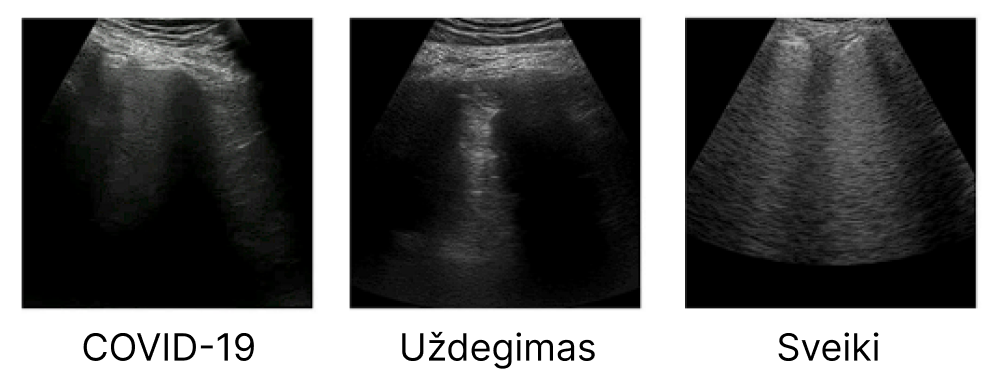
\includegraphics[scale=0.40]{img/plauciai.PNG}
    \caption{Treniravimo echoskopijos vaizdo įrašų kadrų pavyzdžiai \cite{HASAN2023}}
    \label{img:plauciai}
\end{figure}\par
Pasak autorių, plaučių echoskopijos nuotraukose dažnai egzistuoja taškinio triukšmo, gadinančio treniravimo efektyvumą. Šiai problemai išspręsti autoriai panaudojo nuotraukų pakeitimus, kaip kontrasto pakeitimas ir erdvinis filtravimas, kad sumažintų klaidinančius artefaktus. Erdviniui filtravimui autoriai panaudojo Perona-Maliko netiesinį isotropinį metodą, kuris, pagal autorius, nesulieja ir nelokalizuoja nuotraukos, kas svarbu išlaikant nuotraukos turinį, kaip pavyzdžiui jos reikšmių ribos. Pagal autorius, kontrasto pakeitimus reikia naudoti atsargai, nes tai gali sugadinti svarbius požymius nuotraukoje. Tam tikslui autoriai pasinaudojo „Contrast Limited Adaptive Histogram Equalization“ (strumpinus CLAHE, liet. adaptyvusis kontrastu apribotos histogramos išlyginimas) metodu. CLAHE metodas, pagal autorius, apdoroja tik smulkias erdvines lokacijas ir jų rezultatus interpoliuoja, todėl nesukuria naujų defektų nuotraukose. \cite{HASAN2023}

\subsection{Apmokymas}
Autoriai modelių architektūras apmokė su savo kompiuteriniais resursais, naudodami Core i7 procesorių, 16 GB atminties ir Nvidia RTX 2070 Super grafikos plokštę. Autoriai apmokymui ir testavimui naudojo „Tensorflow“ karkasą. Kaip minėta anksčiau, autoriai apmokė ir treniravo VGG16, VGG19, ResNet34, ResNet101, Xception modelius adaptuodami be neapibrėžto sutelkimo ir ištreniruotus su „ImageNet“ rinkiniu, adaptuodami su neapibrėžtu sutelkimu ir pakeičiant visus sutelkimo sluoksnius į neapibrėžto sutelkimo. Autoriai naudojo  \(1 \cdot 10^{-4}\) mokymo žingsnį. Autoriai teigia, jog treniravo modelius iki kol 5 epochas iš eilės metrikos negerėja. \cite{HASAN2023}

\begin{table}[H]\footnotesize
  \centering
\caption{Parametrų kiekis modeliuose, kurių visi sutelkimo sluoksniai neapibrėžti \cite{HASAN2023}}
\begin{tabular}{|l|c|}
\hline
Modelis      & Parametrai  \\ \hline
VGG16      & 15,5 mln.           \\
VGG19      & 20,8 mln.            \\
ResNet34   & 22,09 mln.             \\
ResNet101  & 45 mln.            \\
Xception   & 20,89 mln      \\ \hline
  \end{tabular}
  \label{tab:fuzzyparams}
\end{table}

\subsection{Rezultatai}
Rezultatams atvaizduoti autoriai naudojo „Matthews correlation coefficient“ (sutrumpinus MCC, liet. Matthews koreliacijos koeficientą, žr. formulę \ref{eq:mcc}), tikslumą ir „Cohen's kappa score“ (liet. Koheno kappa įvertinimą). \cite{HASAN2023}
\begin{equation}\label{eq:mcc}
\text{MCC} = \frac{TP \times TN - FP \times FN}{\sqrt{(TP + FP)(TP + FN)(TN + FP)(TN + FN)}}
\end{equation} Kaip minėta ankstesniuose skyriuose, autoriai naudojo 3 strategijas neapibrėžto sutelkimo pritaikymui:
\begin{enumerate}
    \item Adaptuotų modelių metrikos pateiktos \ref{tab:fuzzyiverciai1} lentelėje. Autoriai pastebi, kad pagal metrikas efektyviausias yra Xception tinklas.
    \item Modelių, kurių paskutinį sutelkimo sluoksnį autoriai pakeitė į neapibrėžtojo sutelkimo,  metrikos pateiktos \ref{tab:fuzzyiverciai2} lentelėje. Autoriai pastebi, kad šios strategijos metrikos gavosi šiek tiek geresnės už tik adaptuotų modelių. Mažiausiai pagerėjo VGG19, daugiausiai pagerėjo VGG16. Xception tinklas turi aukščiausias metrikas iš visų tinklų.
    \item Modelių, kurių visus sutelkimo sluoksnius autoriai pakeitė į neapibrėžtojo sutelkimo,  metrikos pateiktos \ref{tab:fuzzyiverciai3} lentelėje. Autoriai pastebi, jog palyginus su ankstesnėmis strategijomis, ši metrikas pagerino daugiausiai. Visų modelių metrikos (išskyrus ResNet34), autorių nuomone, labai pagerėjo. Xception tinklas surinko aukščiausias metrikų reikšmes.
\end{enumerate}\begin{table}[H]\footnotesize
  \centering
\caption{Modelių, kurie tik adaptuoti, metrikos \cite{HASAN2023}}
\begin{tabular}{|l|c|c|c|}
\hline
Modelis      & Tikslumas & MCC   & Koheno kappa \\ \hline
VGG16      & 0.857  & 0.789 &  0.786            \\
VGG19      & 0.901  & 0.853 &  0.851            \\
ResNet34   & 0.904  & 0.856 & 0.855            \\
ResNet101  & 0.922  & 0.883 & 0.882            \\
\textbf{Xception}   & \textbf{0.931}  & \textbf{0.896} & \textbf{0.896}           \\ \hline
  \end{tabular}
  \label{tab:fuzzyiverciai1}
\end{table}

\begin{table}[H]\footnotesize
  \centering
\caption{Modelių, kurių paskutinis sutelkimo sluoksniai apkeistas su neapibrėžtuoju sutelkimu, metrikos \cite{HASAN2023}}
\begin{tabular}{|l|c|c|c|}
\hline
Modelis      & Tikslumas & MCC   & Koheno kappa \\ \hline
VGG16      & 0.888  & 0.832 &  0.832            \\
VGG19      & 0.902  & 0.853 &  0.853            \\
ResNet34   & 0.907  & 0.860 & 0.860           \\
ResNet101  & 0.935  & 0.9003 & 0.903            \\
\textbf{Xception}   & \textbf{0.953}  & \textbf{0.929} & \textbf{0.929}           \\ \hline
  \end{tabular}
  \label{tab:fuzzyiverciai2}
\end{table}

\begin{table}[H]\footnotesize
  \centering
\caption{Modelių, kurių visi sutelkimo sluoksniai apkeisti su neapibrėžtuoju sutelkimu, metrikos \cite{HASAN2023}}
\begin{tabular}{|l|c|c|c|}
\hline
Modelis      & Tikslumas & MCC   & Koheno kappa \\ \hline
VGG16      & 0.93281  & 0.89934 &  0.89917            \\
VGG19      & 0.94695  & 0.92041 &  0.92037            \\
ResNet34   & 0.91214  & 0.86809 & 0.86808            \\
ResNet101  & 0.93927  & 0.90884 & 0.90883            \\
\textbf{Xception}   & \textbf{0.97157}  & \textbf{0.95733} & \textbf{0.95732}           \\ \hline
  \end{tabular}
  \label{tab:fuzzyiverciai3}
\end{table}
\par
Autoriai pastebi, jog efektyviausias yra Xception tinklas klasifikuojant COVID-19, plaučių uždegimo ir sveikų plaučių klases iš turimo duomenų rinkinio - jis aplenkė visus tinklus visose trijose strategijose ir geriausias metrikas pasiekia, kai modelio sutelkimo visi sluoksniai yra neapibrėžtojo sutelkimo. Autoriai teigia, jog jie pagerino Xception tinklą pasitelkdami neapibrėžtojo sutelkimo metodą, leidžiantį sutelkti požymius daug efektyviau, negu įprastos sutelkimo operacijos, kaip argmax. Autorių nuomone, neapibrėžtas sutelkimas yra sudėtingesnis apskaičiuoti, negu įprastos sutelkimo operacijos, todėl yra lėtesnis už įprastas sutelkimo operacijas ir turi daugiau parametrų (žr. \ref{tab:fuzzyparams} lentelę).Tačiau, pasak autorių, sveikatos priežiūroje greitis nėra toks svarbus kaip tikslumas, kuriuo jų architektūra pralenkia kitus sprendimus. \cite{HASAN2023}

\section{Ilgos trumpalaikės atminties neuroninis tinklas}
2021 metų „Pulmonary COVID-19: Learning Spatiotemporal Features Combining CNN and LSTM Networks for Lung Ultrasound Video Classification“ straipsnyje autoriai pristatė naują sprendimą, padedantį jau egzistuojančioms architektūroms efektyviau nustatyti ligas iš echoskopijos. Autoriai panaudojo ilgos trumpalaikės atminties sprendimą (angl. sutrumpinimas LSTM) \cite{LSTM}. Autoriai, kaip ir kitų straipsnių autoriai, teigia, jog palyginus su kitomis plaučių skenavimo priemonėmis, echoskopija yra pigesnė ir efektyvesnė, tačiau reikalauja patyrusio profesionalo. Pasak autorių, nors echoskopijos nuotraukos gali būti labai tikslios diagnozei, profesionalai dažnai susiduria su problema aptinkant sveiko žmogaus echoskopiją. Autoriai teigia, jog naudojant jau ištreniruotus modelius su ilgos trumpalaikės atminties sluoksniais, galima pagerinti diagnozės efektyvumą. \cite{LSTM}
\subsection{Architektūra}
\begin{figure}[H]
    \centering
    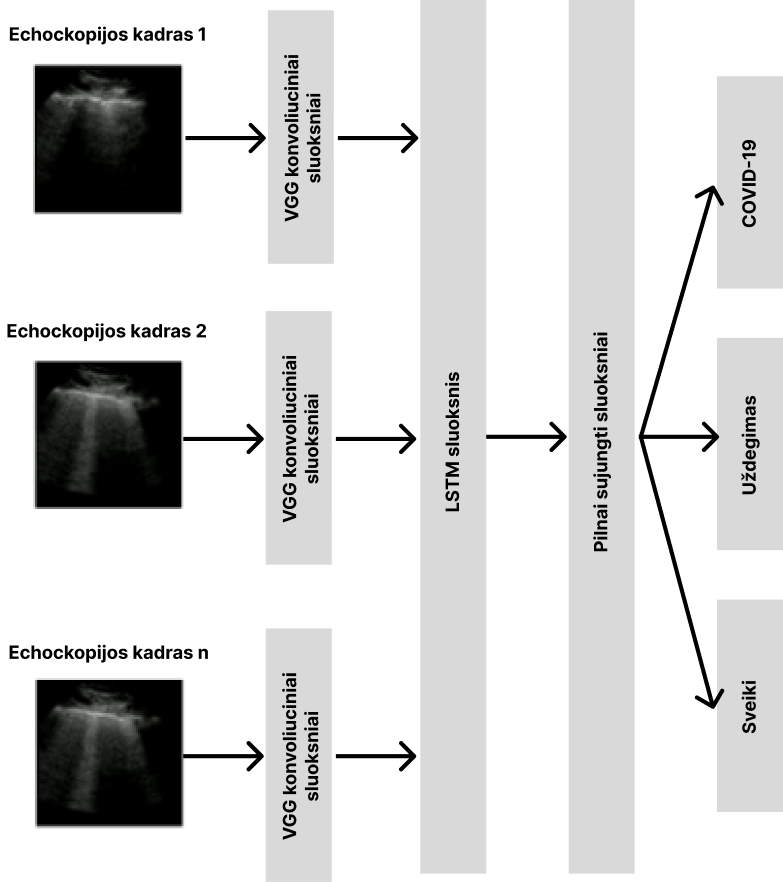
\includegraphics[scale=0.33]{img/lstm.png}
    \caption{Aukšto lygio autorių VGG architektūra \cite{LSTM}}
    \label{img:lstmvgg}
\end{figure}
Autoriai naudojo ilgos trumpos atminties sprendimą, aprašytą \ref{sec:lstm_sub} skyriuje. Pasak autorių, LSTM sprendimas leidžia efektyviai išgauti erdvinę ir laikiną informaciją turinčius duomenis, kurie yra svarbūs vaizdo įrašų klasifikacijos tikslumui. Autoriai pasirinko jų nuomone populiariausias architektūras - VGG, Resnet, Densenet, InceptionV, Inception-ResNetV2, Xception, MobileNet, MobileNetV2 ir EfficientNet ir jas papildė LSTM sluoksniu, dvejais pilnai sujungtų sąryšių sluoksniais su ReLU aktyvacijos funkcija ir išeities sluoksniu su kryžminės entropijos nuostolių funkcija. VGG architektūros pavyzdys iliustruojamas paveikslėlyje \ref{img:lstmvgg}. Autoriai architektūras optimizavo ieškant geriausiai atliekančioms naudojosi hiperparametrų optimizavimo technika (žr. skyrių \ref{sec:apmokymas}) ir vaizdo įrašų kadrų išgavimo konfigūracijomis (žr. skyrių \ref{sec:duomenys}). \cite{LSTM} 
\subsubsection{Ilga trumpa atmintis}\label{sec:lstm_sub}
Pasak straipsnio autorių, ilgos trumpos atminties neuroniniai tinklai gali išspręsti nykstančio gradiento problemą. Tai problema, kuri atsiranda, kai vykstant atgaliniam sklidimui gradientai mažėja iki tiek, kad parametrai mokymosi metu reikšmingai nebe atsinaujina - ilgų sekų, kaip vaizdo įrašų, apdorojimas tampa per sunkus. LSTM naudoja sklendes (angl. „gates“), kurios mokymo metu išmoksta kurias sekas reikia išsaugoti, o kurias atmesti bei ląstelės būseną, saugančią ilgąją atmintį ir paslėptąją būseną, saugančia trumpąją atmintį. LSTM tinklai turi 3 sklendžių tipus: 
\begin{enumerate}
    \item Užmiršimo - reguliuoja atmetamą informaciją būsenos ląstelėje,
    \item Įvesties - reguliuoja pridedamą naudingą informaciją būsenos ląstelėje,
    \item Išvesties - reguliuoja išgaunamą naudingą informaciją iš būsenos ląstelės į išvestį. 
\end{enumerate}

\subsection{Duomenys}\label{sec:duomenys}
Autoriai naudojo atviros prieigos POCUS duomenų rinkinio vaizdo įrašus, kurių iš viso susidarė 185. Vaizdo įrašai priklausė COVID-19, bakterinio uždegimo ir sveikų plaučių klasėms, pasiskirstę beveik po lygiai. Pasak autorių, virusinio uždegimo klasė nebuvo naudota, nes duomenų rinkinyje egzistavo tik 3 vaizdo įrašai su šia liga. Autoriai taip pat surinko artefaktus, rastus duomenų rinkinio vaizdo įrašuose, ir teigia, jog COVID-19 echoskopijos vaizdo įrašuose randama daugiausiai B linijų, bakterinio plaučių uždegimo vaizdo įrašuose daugiausia randama konsolidacijų ir sveikuose plaučiuose daugiausia A linijų.
\par
Autoriai išgavo kadrus iš vaizdo įrašų naudodami skirtingas konfigūracijas - 5, 10, 15 ir 20 išgautų kadrų iš vieno įrašo. Išgautų kadrų pikselių reikšmes autoriai sumažino daugindami iš \(\frac{1}{255}\). Gautų nuotraukų iš kadrų dydis sumažinamas naudojantis interterpoliacijos algoritmu iki \(224 \cdot 244\) su 3 RGB kanalais, kurie pasak autorių reikalingi suderinamumui su „ImageNet“ modeliais.

\subsection{Apmokymas} \label{sec:apmokymas}
Modelius autoriai treniravo ir optimizavo naudodami savo kompiuterinius resursus (Tesla P-100 grafikos plokštę su 16 GB) su TensorFlow karkasu. Treniravimą autoriai atliko su Optuna karkasu, kuris padėjo organizuoti 68 skirtingų modelių optimizaciją ir treniravimą atrenkant geriausius hiperparametrus. Pagal autorius, treniravimas ir optimizacija užtruko \(\approx\)64 valandas. Geriausių modelių hiperparametrai pateikiami \ref{tab:LSTMparams} lentelėje.
\begin{table}[H]\footnotesize
  \centering
\caption{Geriausiai pasirodžiusių modelių su LSTM hiperparametrai\cite{LSTM}}
\begin{tabular}{|l|c|c|c|c|c|c|c|}
\hline
Modelis           & LSTM vienetai   & Atsitiktinis praretinimas   & Mokymo žingsnis  & Parametrų kiekis \\ \hline
Xception-LSTM    &   512               & 0.4                           &  6,55 \cdot \(10^{-4}\)                 & 6,8 mln.           \\
NASNetLarge-LSTM         & 1024               & 0.5                           &  6,62 \cdot \(10^{-4}\)                & 20,8 mln.            \\
DenseNet121-LSTM    & 32               & 0.1                           &  9,08 \cdot \(10^{-4}\)                 & 1,2 mln.             \\
POCOVID-Net-3-LSTM    & 256               & 0.2                           &  8,18 \cdot \(10^{-4}\)                 & 0,8 mln.              \\ 
DenseNet201-LSTM    & 1024               & 0.2                           &  2,54 \cdot \(10^{-4}\)                  & 12,6 mln.              \\ \hline
  \end{tabular}
  \label{tab:LSTMparams}
\end{table}

\par
Autoriai apmokymo metu panaudojo „Cross Validation“ (liet. kryžminės validacijos) sprendimą norėdami užtikrinti modelių generalizaciją \cite{LSTM}. Autoriai padalino duomenų rinkinį į 5 dalis, tai reiškia kad buvo naudojamos 4 dalys treniravimui ir 1 testavimui. Šios dalys pagal šį metodą yra rotuojamos ir po paskutinės dalies, modelis būna treniruotas ir testuotas su visomis dalimis. Galutinis rezultatas buvo skaičiuojamas pasinaudojus visų dalių pasverta suma. Pasak autorių, šis sprendimas padeda išvengti persimokymo, nes su kiekviena dalimi modelis balansuoja rezultatus. 
\subsection{Rezultatai}
Autoriai ištreniravo 68 hibridinius modelius klasifikuoti plaučių echoskopijos vaizdo įrašus. Modelius sudarė CNN ir RNN (rekurentiniai neuroniniai tinklų) modeliai. 1 modelis buvo jau ištreniruotas su nagrinėjamomis klasėmis, 12 modelių treniruoti su „ImageNet“ rinkiniu ir tik pritaikyti nagrinėjamomis klasėmis. Geriausiai pasirodė Xception-LSTM modelis, su 512 LSTM vienetų, 0,4 atsitiktinio praretinimo transformacija ir 20 kadrų seka įvesties sluoksnyje. Autoriai pažymi, jog POCOVID-Net-3-LSTM modelis, kuris paremtas modeliu, skirtu klasifikuoti nagrinėjamoms klasėms, pasiekė vienas aukščiausių metrikų ir beveik pasivijo Xception-LSTM modelį (žr. lentelę \ref{tab:LSTM_rez}). Autoriai teigia, jog  modelių, esančių geriausių lentelėje, metrikos yra geresnės už profesionalaus medicinos darbuotojo, kuris pasak autorių turi 0,546 specifiškumą. \cite{LSTM}
\begin{table}[H]\footnotesize
  \centering
\caption{Geriausiai pasirodžiusių LSTM modelių metrikos \cite{LSTM}}
\begin{tabular}{|l|c|c|c|c|}
\hline
Modelis               & Tikslumas & Precizija   & Specifiškumas     & F1 \\ \hline
Xception-LSTM (20 kadrų)         & 0,93      & 0,94        &  0,97       & 0,93 \\ 
NASNetLarge-LSTM (20 kadrų)      & 0,92      & 0,92     &  0,96          & 0,92  \\
DenseNet121-LSTM (20 kadrų)      & 0,92      & 0,92     &  0,96          & 0,92  \\
POCOVID-Net-3-LSTM (5 kadrų)     & 0,92      & 0,92    & 0,96          & 0,91    \\
DenseNet201-LSTM (5 kadrų)      & 0,92      & 0,91     & 0,96           & 0,92  \\
\hline
  \end{tabular}
  \label{tab:LSTM_rez}
\end{table}

Autoriai taip pat pasinaudojo „Grad-CAM“ technika, kad vizualizuotų Xception-LSTM tinklo išgaunamus požymius su šilumos žemėlapiais. Autoriai palygino klasių artefaktus (žr. \ref{img:plauciai_LSTM} paveikslėlį) ir klasifikacijos šilumos žemėlapių (žr. \ref{img:plauciai_grad}) požymius. Autoriai pastebi, kad uždegimo klasėje šilumos žemėlapis paryškina konsolidacijų vietas, COVID-19 paryškintos B linijos ir netvarkingos pleuros linijos ir sveikuose plaučiuose paryškintos A linijos. Šie modelio išgaunami požymiai, pasak autorių, atitinka medicinines patologijas, naudojamas diagnozuoti šioms ligoms. Autoriai teigia, jog tai rodo, kad modeliai, kurių pagrindas yra ištreniruotas su „ImageNet“, geba puikiai atpažinti ligų požymius echoskopijos nuotraukose.
\begin{figure}[H]
    \centering
    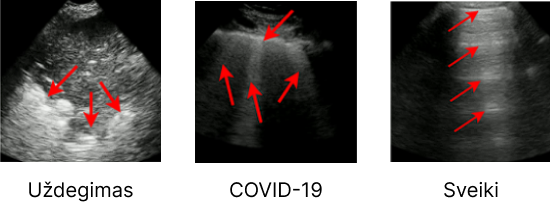
\includegraphics[scale=0.5]{img/Plausiai_ltsm.png}
    \caption{Duomenų rinkinio klasės ir joms būdingi artefaktai. Uždegimui būdingos konsolidacijos, COVID-19 B linijos ir sveikiems A linijos \cite{LSTM}}
    \label{img:plauciai_LSTM}
\end{figure}
\begin{figure}[H]
    \centering
    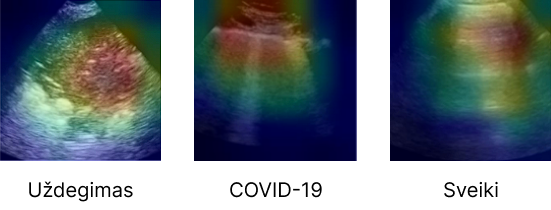
\includegraphics[scale=0.5]{img/plauciai_grad.png}
    \caption{Xception-LSTM šilumos žemėlapiai uždegimo, COVID-19 ir sveikų plaučių echoskopijoms \cite{LSTM}}
    \label{img:plauciai_grad}
\end{figure}

Apibrendrinant rezultatus, autoriai naudodamiesi hiperparametrų optimizacija ir ilgos trumpos atminties technika adaptavo 68 ištreniruotus modelius klasifikuoti vaizdo įrašus į uždegimo, COVID-19 ir sveikų plaučių klases. Geriausiai pasirodė su modelis paremtas Xception architektūra. Autoriai teigia, kad geriausi modeliai gali būti naudojami plaučių ligoms nustatyti dėl jų gerų metrikų.

\sectionnonum{Rezultatai ir išvados}
Šiame darbe apžvelgti giliojo mokymosi sprendimai, galintys medikams padėti nustatyti ligas iš plaučių echoskopijos nuotraukų ir vaizdo įrašų.
\par
Lyginant autorių architektūras, verta paminėti, jog visų straipsnių autoriai tobulino jau sukurtas architektūras šiam uždaviniui spręsti. Transformerių neuroninis tinklas buvo patobulintas su „Linformer“ enkoderiu, konvoliuciniams neuroniniams tinklams buvo pritaikytas neapibrėžtasis sutelkimas, kitas sprendimas konvoliuciniams ir liekanų neuroniniams tinklams pritaikytas įterpiant ilgos trumpalaikės atminties sluoksnį.
\par
Lyginant duomenų rinkinio sprendimus pastebėta, kad visų 3 straipsnių autoriai naudojo tą patį atviros prieigos POCUS duomenų rinkinį ir išgavo kadrus iš vaizdo įrašų, kad treniruotų modelius. LSTM tinklų autoriai naudojosi 4 skirtingomis kadrų išgavimo iš vaizdo įrašų konfigūracijomis, „Fuzzy pooling“ tinklų autoriai naudojo metodus sumažinti triukšmui nuotraukose, o transformerių tinklų autoriai standartizavo visas nuotraukas ir naudojo parametrų balansavimo mechanizmą, kad mažiau nuotraukų turinčios klasės turėtų didesnį svorį. Verta paminėti, jog POCUS duomenų rinkinys yra daug mažesnis už kitus įprastus rinkinius, kaip „Imagenet“, ir jame daugiausiai yra bakterinio uždegimo, COVID-19 ir sveikų plaučių klasių nuotraukų, o kitų ligų duomenų jame trūksta.
\par
Lyginant autorių modelių apmokymus, pastebėta kad visi autoriai apmokė po kelis modelius - transformerių neuroninių tinklų autoriai apmokė 3 dvejų klasių ir 1 daugelių klasių, neapibrėžtojo sutelkimo sprendimo autoriai treniravo 6, o LSTM autoriai 68 modelius. Verta paminėti, jog LSTM autoriai naudojo specialius įrankius optimizuoti hiperparametrus tokiam dideliam kiekiui modelių.
\par
Autorių sukurtų modelių metrikos ir parametrai palyginti lentelėje \ref{tab:palyg}. Pastebėta, jog visų autorių pateikti modeliai turi aukštas metrikas - visos yra intervale tarp 0,8 ir 0,97. Pastebima, kad visi modeliai klasifikavo tik 3 tas pačias diagnozes - COVID-19, bakterinio uždegimo ir sveikų plaučių. LSTM autoriai pristatė plačiau tik geriausiai pasirodusius modelius. Pirmi trys „POCFormer“ modeliai klasifikuoja tik dvi ligas, o likusieji modeliai klasifikuoja 3 diagnozes, todėl auštesnės metrikos gali būti dėl paprastesnio klasifikavimo. Galime pastebėti, jog geriausią tikslumą turi Xception su visais neapibrėžto sutelkimo sluoksniais modelis, tačiau taip pat jis turi ir daugiausia parametrų, kas gali kenkti naudojimui mobiliems echoskopijos įrenginiams su limituota atmintimi. Aukščiausią preciziją turi „POCFormer“ uždegimo ir sveikų plaučių ir Xception-LSTM modeliai, aukščiausią specifiškumą turi Xception-LSTM ir „POCFormer“ COVID-19 ir sveikų plaučių, aukščiausią F1 turi „POCFormer“ daugelio klasių modelis. Mažiausia parametrų turi POCOVID-Net-3-LSTM modelis ir jis išlaiko puikias metrikas. Pastebima, kad neapibrėžto sutelkimo sprendimo autoriai pateikė kitokias metrikas savo modeliams, todėl sunku palyginti su kitų autorių modeliais kitų metrikų atžvilgiu. 
\begin{table}[H]\footnotesize
  \centering
\caption{Modelių palyginimas}
\begin{tabular}{|p{6cm}|c|c|c|c|c|c|c|}
\hline
Modelis & Tikslumas & Precizija & Specifiškumas & F1 & Parametrai \\ \hline
„POCFormer“ COVID-19 ir sveikų plaučių  & 0,91 & 0,87 & 0,97 & 0,92 & 2,8 mln. \\
„POCFormer“ COVID-19 ir uždegimo  & 0,91 & 0,93 & 0,88 & 0,93 & 2,8 mln. \\
„POCFormer“ uždegimo ir sveikų plaučių  & 0,91 & 0,95 & 0,8 & 0,93 & 2,8 mln. \\
„POCFormer“ daugelio klasių  & 0,94 & 0,94 & 0,96 & 0,94 & 6,9 mln. \\
Xception su paskutiniu neapibrėžto sutelkimo sluoksniu  & 0,95 & - & - & - & - \\
Xception su visais neapibrėžto sutelkimo sluoksniais  & 0,97 &-  & - &  -& 20,9 mln. \\
Xception-LSTM  & 0,93 & 0,94  & 0,97 &  0,93 & 6,8 mln \\
NASNetLarge-LSTM  & 0,92 & 0,92  & 0,96 &  0,92 & 20,8 mln \\
DenseNet121-LSTM  & 0,92 & 0,92  & 0,96 &  0,92 & 1,2 mln \\
POCOVID-Net-3-LSTM  & 0,92 & 0,92  & 0,96 &  0,91 & 0,8 mln \\
DenseNet201-LSTM  & 0,92 & 0,91  & 0,96 &  0,92 & 12,6 mln \\
\hline
  \end{tabular}
  \label{tab:palyg}
\end{table}
\par
Visų 3 straipsnių autoriai pateikė modelius, kurie gali tiksliai atlikti 2 ligų ir sveikų plaučių diagnozę, taip padedant medikams, kuriems sunku yra išmokti interpretuoti diagnozę. Pastebėta, kad šie modeliai nebuvo testuoti echoskopijos įrenginiuose ir tai nereiškia kad gali būti naudojami praktikoje dėl kompiuterinių resursų apribojimų. Taip pat, autoriai tyrė tik 2 ligų nustatymą dėl POCUS duomenų rinkinio apribojimų - jame trūksta kitų ligų, kaip virusinis uždegimas, echoskopijos nuotraukų ar vaizdo įrašų. Tai gali būti nepatrauklu medikams, nes plaučių echoskopijos artefaktai gali padėti diagnozuoti daugiau negu 2 ligas.  
% Išvadų ir rekomendacijų dalyje išdėstomi pagrindiniai darbo rezultatai (kažkas
% išanalizuota, kažkas sukurta, kažkas įdiegta), pateikiamos išvados (daromi
% nagrinėtų problemų sprendimo metodų palyginimai, siūlomos rekomendacijos,
% akcentuojamos naujovės).


\printbibliography[heading=bibintoc]  % Šaltinių sąraše abėcėlės tvarka išdėstomi darbe panaudotų
% (cituotų, perfrazuotų ar bent paminėtų) mokslo leidinių, kitokių publikacijų
% bibliografiniai aprašai. Aprašai pateikiami netransliteruoti.

\end{document}
